\documentclass[12pt]{article}
\usepackage[top=1in,left=1.25in,right=1.25in,footskip=1in]{geometry}

\usepackage{graphicx}
\usepackage{xspace}
%\usepackage{adjustbox}

\newcommand{\comment}{}
\renewcommand{\comment}{\nocomment}
\renewcommand{\comment}{\showcomment}

\newcommand{\showcomment}[3]{\textcolor{#1}{\textbf{[#2: }\textsl{#3}\textbf{]}}}
\newcommand{\nocomment}[3]{}

\newcommand{\jd}[1]{\comment{cyan}{JD}{#1}}
\newcommand{\swp}[1]{\comment{magenta}{SWP}{#1}}
\newcommand{\bmb}[1]{\comment{blue}{BMB}{#1}}
\newcommand{\djde}[1]{\comment{red}{DJDE}{#1}}
\newcommand{\old}{\sffamily}
\newcommand{\told}{\textsf}

\newcommand{\eref}[1]{Eq.~\ref{eq:#1}}
\newcommand{\fref}[1]{Fig.~\ref{fig:#1}}
\newcommand{\Fref}[1]{Fig.~\ref{fig:#1}}
\newcommand{\sref}[1]{Sec.~\ref{#1}}
\newcommand{\frange}[2]{Fig.~\ref{fig:#1}--\ref{fig:#2}}
\newcommand{\tref}[1]{Table~\ref{tab:#1}}
\newcommand{\tlab}[1]{\label{tab:#1}}
\newcommand{\pday}{\ensuremath{/\textrm{day}}}

\usepackage{amsthm}
\usepackage{amsmath}
\usepackage{amssymb}
\usepackage{amsfonts}

\usepackage{lineno}
\linenumbers

\usepackage[pdfencoding=auto, psdextra]{hyperref}

\usepackage{natbib}
\bibliographystyle{chicago}
\date{\today}

\usepackage{xspace}
\newcommand*{\ie}{i.e.\@\xspace}

\usepackage{color}

\newcommand{\Rx}[1]{\ensuremath{{\mathcal R}_{#1}}\xspace} 
\newcommand{\Ro}{\Rx{0}}
\newcommand{\Rc}{\Rx{\mathrm{c}}}
\newcommand{\Ri}{\Rx{\mathrm{i}}}
\newcommand{\RR}{\ensuremath{{\mathcal R}}\xspace}
\newcommand{\Rhat}{\ensuremath{{\hat\RR}}}
\newcommand{\Rprop}{\Rx{\mathrm{prop}}}
\newcommand{\Rcori}{\Rx{\mathrm{g0}}}
\newcommand{\tsub}[2]{#1_{{\textrm{\tiny #2}}}}
\newcommand{\dd}[1]{\ensuremath{\, \mathrm{d}#1}}
\newcommand{\dtau}{\dd{\tau}}
\newcommand{\dx}{\dd{x}}
\newcommand{\dsigma}{\dd{\sigma}}

\newcommand{\tstart}{\ensuremath{\tsub{t}{start}}\xspace}
\newcommand{\tend}{\ensuremath{\tsub{t}{end}}\xspace}

\newcommand{\betaeff}{\ensuremath{\tsub{\beta}{eff}}\xspace}
\newcommand{\Keff}{\ensuremath{\tsub{K}{eff}}\xspace}
\newcommand{\Kpost}{\ensuremath{\tsub{K}{post}}\xspace}

\newcommand{\pt}{p} %% primary time
\newcommand{\st}{s} %% secondary time

\newcommand{\psize}{{\mathcal P}} %% primary cohort size
\newcommand{\ssize}{{\mathcal S}} %% secondary cohort size

\newcommand{\gtime}{\sigma} %% generation interval
\newcommand{\gdist}{g} %% generation-interval distribution

\newcommand{\geff}{g_{\textrm{eff}}} %% generation-interval distribution

\newcommand{\total}{{\mathcal T}} %% total number of serial intervals

\newcommand{\PP}{\ensuremath{\mathcal P}}
\newcommand{\II}{\ensuremath{\mathcal I}}
\newcommand{\HH}{\ensuremath{\mathcal H}}

\begin{document}

\begin{flushleft}{
	{\large \textbf{\newline
		Quantifying the effects of strength- and speed-like interventions on epidemic dynamics
	}
	}
}
\newline
\\
Sang Woo Park\textsuperscript{1,*}, Kaiyuan Sun, Benjamin M. Bolker, Bryan T. Grenfell, Jonathan Dushoff, \swp{and others if needed}
\\
\bigskip
\textbf{1} Department of Ecology and Evolutionary Biology, Princeton University, Princeton, NJ, USA
\\
\bigskip

*Corresponding author: swp2@princeton.edu
\end{flushleft}

\section*{Abstract}

needed

\section{Introduction}

The reproduction number \RR---typically defined as the average number of new infections caused by an infected individual---is a key characteristic of an emerging epidemic.
Its value in a fully susceptible population---the \emph{basic} reproduction number, \Ro---provides information about whether a pathogen can invade, the level of intervention required to prevent invasion, and the final size of an epidemic \citep{diekmann1990definition,anderson1991infectious}.
When an epidemic is ongoing, transmission dynamics are affected by changes in population-level immunity, non-pharmaceutical interventions, and contact patterns---these changes in transmission dynamics can be described by $\RR(t)$, often referred to as the \emph{effective} or \emph{time-dependent} reproduction number \citep{wallinga2004different, fraser2007estimating, cori2013new}.
Interpretation and estimation of $\RR(t)$ have been a key area of research during the ongoing COVID-19 outbreaks \citep{pan2020association,flaxman2020estimating,gostic2020practical}.

One of the main challenges in interpreting $\RR(t)$ can be attributed, in part, to its standard, heuristic definition: the average number of new infections caused by an infected individual.
While this definition is biologically intuitive, it is mathematically imprecise as time-dependent reproduction numbers can be defined in multiple ways, depending on the cohort (e.g., a group of individuals who developed symptoms or were infected at the same time) and the types of transmission scenarios (i.e., realized or counterfactual transmission processes).
Here, we primarily focus on two main measures of transmission that look at a cohort of infectees or infectors that were infected at the same time: the instantaneous reproduction number $\Ri(t)$ and the case reproduction number $\Rc(t)$.

The instantaneous reproduction number $\Ri(t)$---popularized by \cite{cori2013new}---was initially defined as the ``average number of people someone infected at time $t$ could expect to infect should conditions remain unchanged'' \citep{fraser2007estimating}. 
While this definition is correct, we note that there are additional subtleties involved:
$\Ri(t)$ does not depend directly on when person gets infected, only on the time point where the ``conditions'' are evaluated.
But transmission conditions always change over the course of an epidemic due to susceptible depletion, and usually for other reasons, meaning that $\Ri(t)$ is a ``counterfactual'' quantity that does not estimate the number of people infected by any particular cohort.
Nonetheless, $\Ri(t)$ is valuable because it provides a way of characterizing transmission conditions at time, and specifically of asking whether the disease would continue to spread if those conditions were to stay the same \citep{gostic2020practical}.

The case reproduction number $\Rc(t)$---popularized by \cite{wallinga2004different}---corresponds to the average number of new infections that an individual infected at time $t$ generated over the course of their infection.
$\Rc(t)$ is a realized measure, which depends on conditions after time $t$ and can only be estimated retrospectively.
Although the heuristic definition of $\RR(t)$ (``the average number of new infections caused by an infected individual'') closely resembles that of $\Rc(t)$, the mathematical definitions of $\RR(t)$ derived from standard compartmental models (e.g., basic reproduction multiplied by the proportion susceptible) actually correspond to that of $\Ri(t)$ \citep{gostic2020practical}.
Hereafter, we use $\RR(t)$ to refer to the instantaneous reproduction number $\Ri(t)$ and return to the distinction between $\Ri(t)$ and $\Rc(t)$ later.

Analogous to the reproduction number $\RR$, exponential growth rate $r$ describes the speed at which infection spreads at the population level.
When conditions remain the same, both $\RR$ and $r$ provide equivalent threshold measures for control and are linked by the generation-interval distribution $g(\tau)$, where generation intervals describe time between infections of an infector and an infectee \citep{svensson2007note}.
Throuhgout the pandemic, most analyses relied on changes in $\RR(t)$ to evaluate the impact of intervention \citep{flaxman2020estimating,brauner2021inferring}.
A few studies have adopted time-varying growth rates $r(t)$ to monitor the spread of infections, but there has been a some controversy about the relative importance of $\RR(t)$ vs.~$r(t)$.
For example, \cite{parag2022} argued that $\RR(t)$ is theoretically more informative than $r(t)$ when the generation-interval distribution is known and underlying assumptions about pathogen transmission hold.
We have argued that they are better seen as complementary measures, with the relative value dependent on what information is available and what interventions are being considered \citep{dushoff2021speed}.

In this study, we extend the strength--speed framework of \cite{dushoff2021speed} to illustrate the differences between $\RR(t)$ and $r(t)$ in characterizing changes in epidemic dynamics.
Here, epidemic ``strength'' and ``speed'' refer to the reproduction number $\RR$ and the growth rate $r$, respectively; 
in parallel, we use ``constant-strength'' and ``constant-speed'' interventions to refer to idealized interventions that directly affect $\RR$ and $r$, respectively. 
For example, a constant-strength intervention that reduces the transmission rate by a constant amount $\theta$ throughout infection can control the epidemic when $\theta > \RR$. 
Analogously, a constant-speed intervention that isolates infected individuals at a constant rate $\phi$ throughout infection can control the epidemic when $\phi > r$.
We note that these idealized interventions are assumed to be constant across time of infection, but not necessarily across calendar time--- we can imagine constant-strength and -speed interventions whose effectiveness can vary throughout an epidemic.

We begin by showing that the renewal process of infection can be expressed in two equivalent ways using instantaneous and case-based perspectives.
The first renewal equation relies on the instantaneous reproduction number $\Ri(t)$, and therefore connects past and current incidence using a counterfactual distribution, which we call the instantaneous generation-interval distribution.
The second renewal equation relies on the case reproduction number $\Rc(t)$, a realized measure of transmission, and therefore connects past and current incidence using a realized distribution, which we call the forward generation-interval distribution.
Instantaneous and forward generation-interval distributions differ qualitatively in the way they change through time.
For example, a constant-strength intervention causes the forward distribution to change over time even though the instantaneous distribution remains invariant.
On the other hand, a constant-speed intervention causes both distributions to change, which must be taken into account to correctly estimate $\Ri(t)$ and $\Rc(t)$.
Instead, the time-varying growth rate $r(t)$ is a robust measure for changes in incidence under both constant-strength and constant-speed interventions as it does not require assumptions about the underlying distribution.
Finally, we use a simple SIR model as an example to demonstrate that changes in the transmission rate are equivalent to a constant-strength intervention, whereas changes in the recovery rate are equivalent to a constant-speed intervention;
we note that the renewal equation theory can be generalized to more complex class of models \citep{champredon2018equivalence}.
We conclude that $\RR(t)$ is generally a better measure for characterizing disease spread under constant-strength interventions, whereas $r(t)$ is generally better under constant-speed interventions.

\section{Mathematical theory}

\subsection{Renewal equation framework}

The renewal-equation framework provides a flexible way of modeling the spread of infection and the impact of intervention \citep{fraser2007estimating}.
Let $K(t, \tau)$ represent the infection kernel, defined as the rate at which secondary cases are generated at time $t$ by an individual infected $\tau$ time units ago (we will use $s, t$ to denote calendar time and $\sigma, \tau$ to denote time since infection).
The shape of this kernel can depend on characteristics of the infection (e.g., variation in infectiousness over the course of infection) as well as other population-level factors (e.g., susceptible depletion, non-pharmaceutical interventions, and changes in behavior).
Then, incidence of infection at time $t$ caused by a cohort of individuals infected $\tau$ time units ago can be written as the product of the kernel, $K(t, \tau)$, and incidence at time $t-\tau$, $i(t-\tau)$:
\begin{equation}
i_{t-\tau}(t) = K(t, \tau) i(t-\tau).
\end{equation}
Integrating across time since infection $\tau$ allows us to express the dynamics of incidence $i(t)$ using a renewal-equation framework: 
\begin{align}
i(t) &= \int_0^\infty K(t, \sigma) i(t-\sigma) \dsigma.
\label{eq:renewal}
\end{align}
This formulation generalizes the dynamics of many compartmental models, including the standard SIR and SEIR models \citep{heesterbeek1996concept, diekmann2000mathematical, roberts2004modelling, aldis2005integral, roberts2007model, champredon2018equivalence}.
Throughout this paper, we focus on changes in infection and ignore complexities associated with observing infections, such as delays between infection and case reports.

Here, we show that the dynamics of this infection model can be expressed equivalently in terms of instantaneous quantities or in terms of realized quantities, meaning $\Ri(t)$ and $\Rc(t)$ with their corresponding generation-interval distributions.
The integral of $K(t, \tau)$ across $\tau$ with $t$ fixed gives the instantaneous reproduction number \citep{fraser2007estimating}: $\Ri(t) = \int K(t, \sigma) \dsigma$.
If we normalize this kernel, we get the instantaneous generation-interval distribution $g_t(\tau) = K(t, \tau)/\Ri(t)$.
The instantaneous reproduction number and generation-interval distribution describe (counterfactual) quantities that would be realized only if conditions remained constant (i.e., if $K(s, \tau) = K(t, \tau)$ for all $s \geq t$).
The renewal equation (\eref{renewal}) can be rewritten using this decomposition:
\begin{align}
i(t) &= \Ri(t) \int_0^\infty g_t(\sigma) i(t-\sigma) \dsigma.
\label{eq:renewal_instantaneous}
\end{align}
For example, if disease parameters remain constant in a simple model, such as the SEIR model, we would expect $\Ri(t) = \Ro S(t)$ and $g_t(\tau) = g_0(\tau)$, where $g_0(\tau)$ represents the intrinsic generation-interval distribution \citep{champredon2015intrinsic}.

Now, consider the forward kernel $F_t(\tau)$, which represents the rate at which an individual infected at time $t$ generates secondary infections $\tau$ time units after infection: 
\begin{equation}
F_t(\tau) = K(t+\tau, \tau).
\label{eq:fkernel}
\end{equation}
The integral of $F_t(\tau)$, representing the total infectiousness of an individual infected at time $t$, corresponds to the case reproduction number: $\Rc(t) = \int F_t(\sigma) \dsigma$. 
The forward kernel, normalized by the total infectiousness, corresponds to the forward generation-interval distribution $f_t(\tau) = F_t(\tau)/\Rc(t)$, describing realized generation intervals for a cohort of infectors that were infected at time $t$.
Then, the forward renewal equation can be written as:
\begin{align}
i(t) &= \int_0^\infty \Rc(t-\sigma) f_{t-\sigma}(\sigma) i(t-\sigma) \dsigma.
\label{eq:renewal_forward}
\end{align}
This forward renewal equation provides an equivalent description of the infection processes as the instantaneous form (\eref{renewal_instantaneous}).

We can check that the instantaneous quantities ($\Ri(t)$ and $g_t(\tau)$) match the forward realized quantities ($\Rc(t)$ and $f_t(\tau)$) when conditions remain constant (or effectively constant, as in the case of early exponential spread).
Assuming that $K_s(\tau) = K_t(\tau)$ for all $s \geq t$, we obtain $F_{t}(\tau) = K(t, \tau)$ (and therefore, $\Rc(t) = \Ri(t)$ and $f_{t}(\tau) = g_t(\tau)$).

\subsection{Constant-strength and constant-speed interventions}

To model changes in epidemic dynamics, we introduce an intervention function $\II(t, \tau)$ which can depend on both calendar time $t$ as well as time since infection $\tau$. 
Then, the infection kernel under $\II$ at calendar time $t$ can be written as:
\begin{equation}
K(t, \tau) = \Ro \II(t, \tau) g_0(\tau),
\end{equation}
where $g_0$ is the pre-intervention instantaneous generation interval (assumed to remain nearly constant for the time period of interest, apart from the effects of the intervention)
The forward kernel of an individual infected at time $t$ under $\II$ can then be written as:
\begin{equation}
F_t(\tau) =  \Ro \II(t + \tau, \tau) g_0(\tau).
\end{equation}
The intervention function $\II(t, \tau)$ can capture any kinds of epidemiological changes, including changes in the susceptible pools $S(t)$ (either due to natural infection or vaccination) as well as introduction and lifting of non-pharmaceutical interventions.

We focus on two idealized interventions, which we refer to as constant-strength and constant-speed interventions, and later generalize them \citep{dushoff2021speed}.
While our primary focus is on the instantaneous quantities ($\Ri(t)$ and $g_t(\tau)$), we first illustrate the impact of constant-strength and constant-speed interventions using forward quantities as they describe realized transmission processes and are easier to interpret.
In particular, the forward kernel allows us to describe how intervention measures will affect onward transmisison of an infected individual.
We present the impact of these idealized interventions on instantaneous kernels in Supplementary Materials. 
as we explain later, the impact of intervention measures on instantaneous kernel can be counterintuitive.

\begin{figure}[!th]
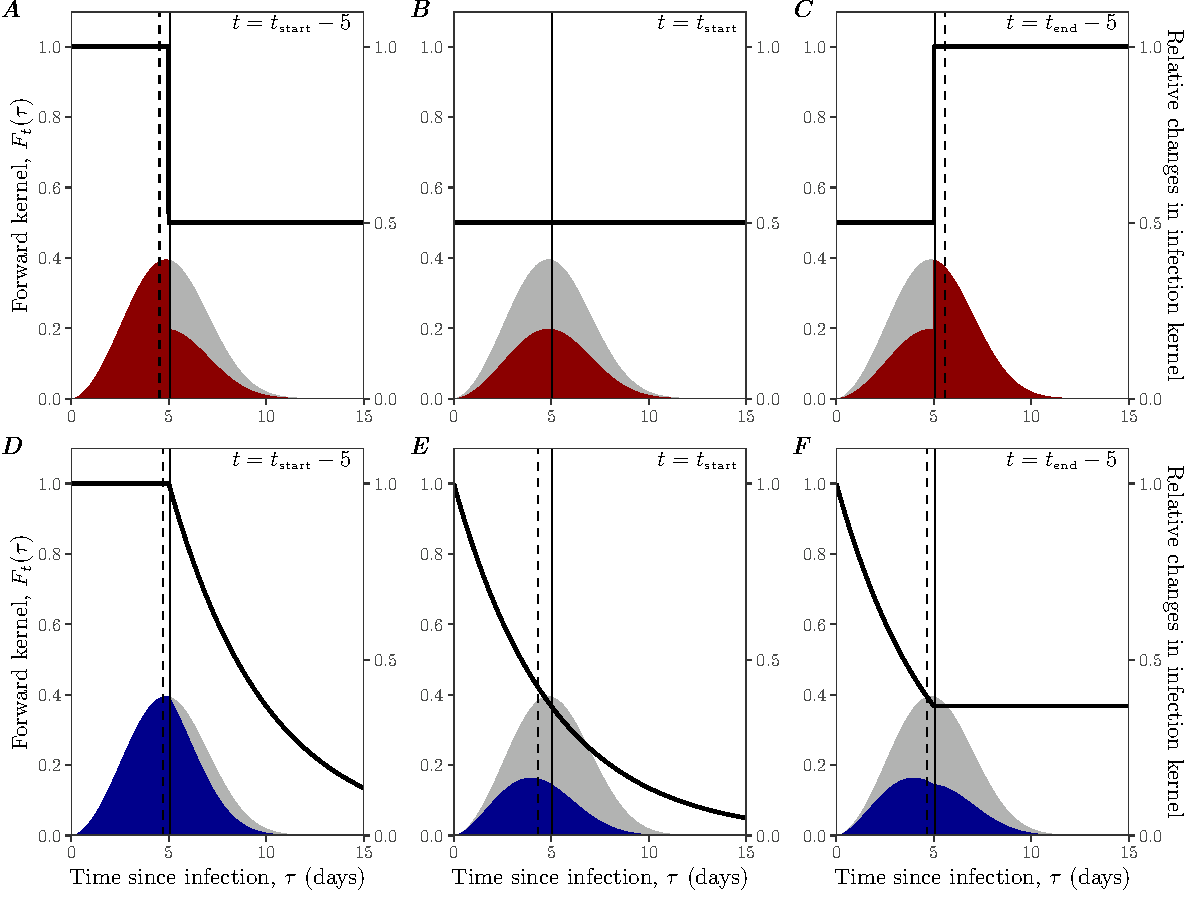
\includegraphics[width=1\textwidth]{pop_ind_compare.pdf}
\caption{
\textbf{The impact of constant-strength and constant-speed interventions on forward kernels.}
The impact of constant-strength (A--C) and constant-speed (D--F) intervention on forward kernels of cohort of individuals infected at different time:
5 days before intervention onset (A, D), during intervention (B, E), and 5 days before intervention offset (C, F).
Gray shaded curves represent the (fixed) intrinsic kernel $K_0(\tau)$, which is modeled using a gamma distribution with $\Ro$ of 2, a mean of 5 days and a squared coefficient of variation of 0.2.
Colored curves represent the forward kernel $F_t(\tau)$ under constant-strength (A--C) and constant-strength (D--F) interventions.
The constant-strength intervention is assumed to reduce kernel by a factor of 2.
The constant-speed intervention is assumed to have a constant hazard of $1/5/\textrm{days}$ during the intervention period.
Susceptible depletion is assumed to be negligible.
Solid black lines represent relative changes in the kernel: $F_t(\tau)/K_0(\tau)$.
Solid vertical lines show the (fixed) mean intrinsic generation interval and dashed vertical lines the mean forward generation interval.
See Supplementary Figure S1 for the impact of constant-strength and constant-speed interventions on instantaneous kernels.
}
\label{fig:indpop}
\end{figure}

First, we consider a constant-strength intervention $\II(t, \tau) = \PP(t)$, which reduces the transmission rate by a constant amount across the age of infection $\tau$ at a given time $t$; note that $\PP(t)$ need not be constant across calendar time.
In particular, the forward kernel corresponds to $F_t(\tau) =  \Ro \PP(t+\tau) g_0(\tau)$, and therefore changes in intervention $\PP$ across calendar time will affect the shape of the forward kernel.
For example, a constant-strength intervention that reduces transmission by a factor of $\theta$ between time \tstart and \tend can be modeled as:
\begin{equation}
\PP(t) = \begin{cases}
1 & t < \tstart\\
\frac{1}{\theta} & \tstart \leq t < \tend\\
1 & \tend \leq t
\end{cases}.
\end{equation}
\fref{indpop}A--C illustrates the impact of such intervention on the forward kernel $F_t(\tau)$ of an individual infected 5 days before $\tstart$, 5 days after $\tstart$, and 5 days before $\tend$.
This constant-strength intervention reduces transmission immediately (\fref{indpop}A);
likewise, lifting this intervention can, in theory, cause the forward kernel to return back to normal immediately (\fref{indpop}C).
Even though the exact shape of the kernel $F_t(\tau)$ depends on the time of infection and when the intervention was introduced relative to the infection time, the relative impact of intervention in reducing transmission (black solid lines in \fref{indpop}A--C, representing $F_t(\tau)/K(0, \tau)$) is constant ($1/\theta$) for transmission that occurs during the intervention period.

Such intervention has predictable effects on forwarrd generation intervals:
implementing (lifting) intervention decreases (increases) future transmission potential and therefore decreases (increases) the mean forward generation interval (\fref{indpop}A,C).
If an individual is infected after \tstart (and much earlier than \tend), this intervention simply reduces the entire kernel by a constant amount and has no effect on realized generation intervals (\fref{indpop}B).
This observation generalizes the phenomenon of contraction of realized generation intervals due to susceptible depletion \citep{kenah2008generation,nishiura2010time,champredon2015intrinsic}.

On the other hand, the instantaneous kernel at time $t$ corresponds to $K(t, \tau) = \Ro \PP(t) g_0(\tau)$, and changes in $\PP$ before or after time $t$ (e.g., onset or offset of intervention) does not affect the shape of $K(t, \tau)$.
Therefore, before the intervention is introduced, the instantaneous kernel is identical to the intrinsic kernel (Supplementary Figure S1A).
During the intervention, the constant-strength intervention reduces the overall height of the kernel by a factor of $\theta$ but does not affect its shape otherwise (Supplementary Figure S1B--C).
In other words, the onset and offset of constant-strength intervention does not affect the shape of the instantaneous generation-interval distribution---this property allowed previous studies to conclude that $\Ri(t)$ should be estimated with an intrinsic generation-interval distribution \citep{gostic2020practical}.

Analogously, we consider a constant-speed intervention $\II(t, \tau) = \HH(t, \tau)$ that depends on time-varying hazard of isolation $h(t)$:
\begin{equation}
\HH(t, \tau) = \exp \left(- \int_0^\tau h(t-\sigma) \dsigma \right).
\end{equation}
Analogous to the constant-strength intervention, the constant-speed intervention assumes a constant hazard of isolation across the age of infection $\tau$ at a given time $t$; however, the hazard need not be constant across calendar time.
Then, $\HH(t,\tau)$ represents the probability that an individual infected $\tau$ time units ago has not been isolated by calendar time $t$.
In practice, the hazard of isolation is expected to depend not only on calendar time $t$ but also on the age of infection $\tau$---for example, we expect $h(t, \tau)$ to increase with $\tau$ for symptom-based interventions to reflect the increasing cumulative probability of developing symptoms.

For example, a constant-speed intervention that takes place between time \tstart and \tend can be modeled using the following hazard function:
\begin{equation}
h(t) = \begin{cases}
0 & t < \tstart\\
\phi & \tstart \leq t < \tend\\
0 & \tend \leq t
\end{cases}.
\end{equation}
Since the forward kernel corresponds to $F_t(\tau) =  \Ro \HH(t+\tau, \tau) g_0(\tau)$, the probability that an individual infected at time $t$ has not been isolated by $\tau$ time units after infection depends on the amount of time the individual has been exposed to this intervention.
If the individual is infected before $\tstart$, they will not be isolated by this intervention until after $\tstart$.
If the individual is infected after $\tend$, they will never be isolated by this intervention.
\fref{indpop}D--F illustrates the impact of such intervention on the forward kernel of an individual infected 5 days before $\tstart$, at $\tstart$, and 5 days before $\tend$.
Unlike the constant-strength intervention, the constant-speed intervention does not show effects immediately;
that is, the rate at which an infected individual generates secondary infections at time $\tstart$ remains unaffected by the intervention because it takes time to identify and isolate infected individuals.
On the other hand, when the intervention is lifted at $\tend$, the value of the kernel at calendar time remains unchanged because some fraction of infected individuals have already been isolated.
Constant-speed interventions always shorten realized generation intervals because they prevent late transmission (\fref{indpop}D--F).

The effect of constant-speed intervention on the instantaneous kernel, $K(t, \tau) = \Ro \HH(t, \tau) g_0(\tau)$, is less obvious.
For individuals infected at time $t$, the forward kernel $F_t(\tau)$ depends on the hazard between time $t$ and $t+\tau$ because $F_t(\tau)$ describes conditions \emph{after} time $t$.
On the other hand, the instantaneous kernel $K(t, \tau)$ depends on the hazard between time $t-\tau$ and $t$ because $K(t, \tau)$ describes conditions \emph{at} time $t$.
Once again, before the constant-speed intervention is introduced, the instantaneous kernel is identical to the intrinsic kernel (Supplementary Figure S1D).
During intervention, in particular when $t=\tstart+x$, the instantaneous kernel reflects the first $x$ days of constant-speed intervention effort:
therefore, $K(t,\tau)/K(0, \tau)$ decreases for the first $x$ days and plateaus (Supplementary Figure S1E--F).
Constant-speed interventions also always shorten instantaneous generation intervals---we show later that the timing of reduction in forward and instantaneous generation intervals differs.

Finally, we can decompose the generalized intervention function $\II(t, \tau)$ as a product of constant-strength and constant-speed interventions: $\II(t, \tau) = \PP(t) \HH(t, \tau)$.
In this case, the forward kernel corresponds to:
\begin{equation}
F_t(\tau) = \Ro \PP(t+\tau) \HH(t+\tau, \tau) g_0(\tau),
\end{equation}
which can be used to describe the dynamics of incidence $i(t)$ in the form of \eref{renewal_forward}.  
Likewise, the instantaneous kernel corresponds to: 
\begin{equation}
K(t, \tau) = \Ro \PP(t) \HH(t, \tau) g_0(\tau),
\end{equation}
which can be used to describe the dynamics of incidence $i(t)$  in the form of \eref{renewal_instantaneous}.
In both case, the combined effects of constant-strength and constant-speed intervention can be understood in terms of the product of their marginal effects.

\subsection{Quantifying changes in generation-interval distributions}
\label{ss:instg}

In order to model the renewal process and accurately estimate $\Ri(t)$, we have to know how the instantaneous generation-interval distribution $g_t(\tau)$ changes across time $t$.
The instantaneous distribution measures the infectiousness of an individual infected $\tau$ time units ago at time $t$ and is therefore different from the distribution of realized generation intervals (i.e., time between actual infection events).
For example, while both the forward generation-interval distribution $f_{t-\tau}(\tau)$ and the instantaneous generation-interval distribution $g_t(\tau)$ depend on the rate at which secondary cases at time $t$ are generated by a primary case infected at time $t-\tau$, $K(t, \tau)$, they are normalized by different quantities:
\begin{equation}
f_{t-\tau}(\tau) = \frac{K(t,\tau)}{\int_0^\infty K(t-\tau+\sigma,\sigma) \dsigma} \neq \frac{K(t,\tau)}{\int_0^\infty K(t,\sigma) \dsigma} = g_t(\tau).
\end{equation}
The forward distribution $f_{t-\tau}(\tau)$ is normalized by the average number of new infections caused by an individual infected at time $t-\tau$ (i.e., the case reproduction number, $\Rc(t-\tau)$).
On the other hand, the instantaneous distribution $g_t(\tau)$ is normalized by a counterfactual measure of transmission $\Ri(t)$.

Rewriting \eref{fkernel} provides further insight into their differences:
\begin{equation}
f_t(\tau) = \frac{\Ri(t + \tau) g_{t+\tau}(\tau)}{\int \Ri(t + \sigma) g_{t+\sigma}(\sigma) \dsigma}.
\end{equation}
Even if the instantaneous generation-interval distribution $g_t(\tau)$ remains invariant across calendar time $t$, changes in transmission conditions (and therefore $\Ri(t)$) can change the shape of the forward generation-interval distribution.
For example, as we showed earlier, the forward generation-interval distribution changes under a constant-strength intervention even though the instantaneous generation-interval distribution does not.
Therefore, renewal equation models that rely on the forward form (\eref{renewal_forward}) with time-invariant $f_t(\tau)$ but changing \Rc\ should generally be avoided.

On the other hand, if we were to take all realized generation intervals that end at time $t$ and form a distribution, we obtain what is known as the backward generation-interval distribution, $b_t(\tau)$:
\begin{equation}
b_t(\tau) = \frac{i_{t-\tau}(t)}{\int_0^\infty i_{t-\sigma}(t) \dsigma}.
\label{eq:backward}
\end{equation}
The backward distribution systematically differs from the instantaneous distribution:
\begin{equation}
b_t(\tau) = \frac{g_t(\tau) i(t-\tau)}{\int_0^\infty g_t(\sigma) i(t-\sigma) \dsigma}
\label{eq:b1}
\end{equation}
due to its dependence on previous incidence of infection.
For example, when incidence is increasing exponentially, we are more likely to observe shorter generation intervals for a cohort of infectees that were infected at the same time because their infectors are more likely to have been infected recently.

Rewriting \eref{b1} in terms of the forward distribution shows that the backward distribution also depends on the case reproduction number $\Rc(t-\tau)$ of the cohort of infectors at time $t-\tau$:
\begin{equation}
b_t(\tau) = \frac{\Rc(t-\tau) f_{t-\tau}(\tau) i(t-\tau)}{\int_0^\infty \Rc(t-\sigma) f_{t-\sigma}(\sigma) i(t-\sigma) \dsigma}.
\label{eq:b2}
\end{equation}
As defined in \eref{backward}, the total density of generation intervals between time $t-\tau$ and time $t$ corresponds to $i_{t-\tau}(t)$ (i.e., the total number of infections at time $t$ caused by a cohort of individuals that were infected at time $t-\tau$), which depends on the incidence $i(t-\tau)$ at time $t-\tau$ as well as their average infectiousness $\Rc(t-\tau)$.
In other words, a cohort of infectors that generated more infections will have greater contribution towards the backward generation-interval distribution at a given time.
Several studies have noted, in various contexts, that backward distributions of epidemiological delays provide biased estimates of the forward distribution due to effects of this sort \citep{nishiura2010time,champredon2015intrinsic,park2020forward}.

\subsection{Quantifying changes in reproduction numbers}

The instantaneous reproduction number $\Ri(t)$ provides a measure for the impact of intervention:
%%
\begin{align}
\Ri(t) &= \int_0^\infty K(t, \sigma) \dsigma, \\
&= \RR_0 S(t) \PP(t) \int_0^\infty \HH(t,\sigma) g_0(\sigma) \dsigma.
\label{eq:rt}
\end{align}
%%
Since $\Ri(t)$ measures conditions at time $t$, one would typically expect to detect changes in $\Ri(t)$ as soon as interventions are implemented---as we see in \eref{rt} (and also in \fref{indpop}), this is true for changes in a constant-strength intervention $\PP(t)$ but not under a constant-speed intervention $\HH(t, \sigma)$.
Therefore, it has been previously argued that $\Ri(t)$ can provide a real-time measure for whether the disease will continue to spread or not \citep{gostic2020practical}.

Estimating $\Ri(t)$ depends on the instantaneous generation-interval distribution $g_t(\tau)$,
which can vary across time under constant-speed interventions:
\begin{equation}
g_t(\tau) = \frac{K(t, \tau)}{\RR(t)} = \frac{\HH(t,\tau) g_0(\tau)}{\int_0^\infty \HH(t,\sigma) g_0(\sigma) \dsigma}.
\end{equation}
By rearranging \eref{renewal}, we obtain the following estimator for $\RR(t)$:
\begin{equation}
\Ri(t) = \frac{i(t)}{\int_0^\infty g_t(\sigma) i(t-\sigma) \dsigma}.
\end{equation}
While this estimator is similar in form to previously proposed estimators \citep{fraser2007estimating}, it differs in allowing for the underlying instantaneous generation-interval distribution to vary across time.
In particular, the popular R package \texttt{EpiEstim} uses this approach while assuming that the underlying instantaneous distribution does not change over time \citep{cori2013new};  
such methods can accurately estimate changes in $\Ri(t)$ under constant-strength interventions, but not necessarily under more general conditions.

When both strength- and speed-like interventions are present during an ongoing epidemic, classical estimators \citep{fraser2007estimating,cori2013new} measure a slightly different quantity:
\begin{equation}
\Rcori(t) = \frac{i(t)}{\int_0^\infty g_0(\sigma) i(t-\sigma) \dsigma}.
\end{equation}
This is the number of infections per infection required to explain current incidence under the counter-factual that the generation-interval distribution has not changed.
This estimator is widely used, because it is simple, often robust to estimate, and often a good proxy for \Ri.
When interventions have speed-like components, however, the exact meaning of this estimator can be difficult to interpret; 
and it does not necessarily accurately reflect how conditions are changing through time.

The case reproduction number $\Rc(t)$ is similarly complicated. 
Since $\Rc(t)$ measures the average number of new infections caused by an individual infected at time $t$, we have
\begin{equation}
\Rc(t) = \frac{\int_0^\infty i_t(t+\sigma) \dsigma}{i(t)},
\end{equation}
where $i_t(t+\sigma)$ represents incidence at time $t+\sigma$ caused by individuals who were infected at time $t$.
Substituting \eref{backward}, it is straightforward to see that $\Rc(t)$ can be estimated by using the backward generation-interval distribution:
\begin{equation}
\Rc(t) = \frac{\int_0^\infty b_{t+\sigma}(\sigma) i(t+\sigma) \dsigma}{i(t)}.
\end{equation}
Here, the numerator, which represents the total number of infections caused by individuals infected at time $t$, is calculated by multiplying future incidence $i(t+\sigma)$ with the probability that future infections are caused by an individual infected at time $t$ $b_{t+\sigma}(\sigma)$.
Using \eref{b1}, we obtain a Wallinga-Teunis-like estimator \citep{wallinga2004different}:
\begin{equation}
\Rc(t) = \int_0^\infty \left(\frac{g_{t+\sigma}(\sigma) i(t+\sigma)}{\int_0^\infty g_{t+\sigma}(\sigma') i(t+\sigma-\sigma') \dsigma'} \right) \dsigma.
\label{eq:wtlike}
\end{equation}
This derivation clarifies that, like the classic estimator for \Ri, the classic estimator for \Rc\ is based on the intrinsic generation-interval distribution, and thus implicitly relies on the assumption that changes in transmission are strength-like and not speed-like.

Some studies have suggested substituting the forward distribution $f_t(\tau)$ instead to estimate the ``time-varying'' or the ``effective'' reproduction number $\RR(t)$ \citep{liu2018measurability, ali2020serial}:
\begin{equation}
\tsub{\RR}{forward}(t) = \frac{i(t)}{\int_0^\infty i(t-\sigma) f_{t-\sigma}(\sigma) \dsigma}.
\end{equation}
This choice is potentially problematic, as the forward distribution differs systematically from the instantaneous distribution.
For example, under constant-strength interventions, the forward distribution changes over time even though the instantaneous distribution remains time invaraint---these differences can lead to systematic biases.
In Section 3, we compare $\tsub{\RR}{forward}(t)$ with $\Ri(t)$ and $\Rc(t)$.

\subsection{Quantifying changes in time-dependent growth rate}

The instantaneous reproduction number $\Ri(t)$ provides a long-term threshold for whether the epidemic will \emph{eventually} grow or decline if current conditions remain unchanged;
perhaps counterintuitively, it does not tell us whether the epidemic is growing or not at a given moment.
In contrast, the epidemic growth rate $r(t)$ does provide a convenient metric that is consistent with whether incidence is increasing or decreasing at a given time.
Researchers often focus on the initial exponential growth rate, but we can look at the per-capita growth rate at any time:
\begin{equation}
r(t) = \frac{1}{i(t)} \frac{\dd{i(t)}}{\dd{t}}.
\end{equation}
By definition, incidence grows when $r(t) > 0$ (and vice versa)---thus, this provides an instantaneous threshold for incidence of infection (but does not provide information about the long-term behavior).

\section{Example: Semi-mechanistic SIR model}

In order to understand how constant-strength and constant-speed interventions affect disease spread, we use a semi-mechanistic SIR model to generate synthetic data and compare various estimates of $\RR(t)$ and $r(t)$:
\begin{align}
\frac{\dd{S}}{\dd{t}} &= - \beta(t)S I, \label{eq:dSdt}\\
\frac{\dd{I}}{\dd{t}} &= \beta(t)S I - \gamma(t) I,\\
\frac{\dd{R}}{\dd{t}} &= \gamma(t) I,  \label{eq:dRdt}
\end{align}
where $S$, $I$, $R$ represent the proportion of individuals that are susceptible, infected, and removed (either due to recovery or isolation measures);
$\beta(t)$ represents a time-varying transmission rate; and $\gamma(t)$ represents a time-varying removal rate.
We refer to this model as semi-mechanistic because the infection and recovery process are modeled explicitly, but changes in $\beta$ and $\gamma$ are allowed to change freely over time (without any mechanisms).
In this case, the instantaneous kernel can be written as:
\begin{equation}
K(t, \tau) = \beta(t) S(t) \exp\left(-\int_{t-\tau}^t \gamma(s) \dd{s} \right).
\end{equation}
Thus, changes that affect only the transmission rate $\beta(t)$ (respectively, removal rate $\gamma(t)$) exactly match the definition of constant-strength (constant-speed) interventions.
Note also that an abrupt change in $\beta$ will produce a parallel abrupt change in the kernel, and thus in incidence, while an abrupt change in $\gamma(t)$ will not have an immediate effect, due to delays in isolating individuals.
Finally, the instantaneous reproduction number is given by:
\begin{equation}
\Ri(t) = \beta(t) S(t) \int_0^\infty \exp\left(-\int_{t-\tau}^t \gamma(s) \dd{s} \right) \dtau.
\end{equation}

When $\gamma(t) \equiv \gamma(0)$, we obtain a familiar form: $\Ri(t) = \Ro S(t)$,
where $\Ro = \beta(0)/\gamma(0)$.

\jd{There's a weird subtlety here that we should discuss. It is not obvious how to define the instantaneous kernel, right? It seems possible to argue either for or against the idea that the instantaneous reproduction number is always $\beta(t)/\gamma(t)$ in the SIR. I guess it comes down to whether Fraser's “conditions” refer to $\gamma$ or to $f$ in this case?}
\swp{Pretty sure we've talked about this before. Defining intantaneous kernel also seems obvious to me... in particular, this instantaneous kernel is going to properly link the renewal equation and also give the correct forward kernel. $\beta(t)/\gamma(t)$ is sensitive to sudden changes in $\gamm$ which is not what's happening to transmission.}
\jd{Sure. The problem is that this version doesn't actually describe what is happening “at the instant”. I'm assuming you get that saying $1/\gamma$ is the same as saying “replace $\gamma(s)$ with $\gamma(t)$”. I think it's just solved by text. I was trying to just solve it by editing, but we talk quite a lot about “current conditions”, and this $R_i$ doesn't really match what we say about what would happen if conditions stayed like now. More like if transmission stayed like now, and recovery kept paradoxically mimicking the recent past.} 

\begin{figure}[!ht]
\includegraphics[width=\textwidth]{figure_beta_gamma.pdf}
\caption{
\textbf{Assumed changes in transmission and removal rate.}
The semi-mechanistic SIR model is simulated under two different scenarios.
(A) Equivalent constant-strength intervention scenario.
Removal rate $\gamma$ is fixed to $0.2\pday$ throughout.
(B) Equivalent constant-speed intervention scenario.
Transmission rate $\beta$ is fixed to $0.3\pday$ throughout.
(C) Instantaneous incidence under equivalent constant-strength and constant-speed intervention scenarios (both scenarios give identical incidence trajectories).
(D) Growth rate estimates over time.
}
\label{fig:assumption}
\end{figure}

Here, we compare two different scenarios, in which interventions are introduced and are later partially lifted (\fref{assumption}): one a smooth introduction and lifting of a constant-strength intervention, modeled by changing in $\beta$ while fixing $\gamma$ (\fref{assumption}A); the other a sudden introduction and lifting of a constant-speed intervention, modeled by changing in $\gamma$ while fixing $\beta$ (\fref{assumption}B).
We construct these two to give identical incidence curves (\fref{assumption}C), and thus refer to them as \emph{equivalent} interventions.
This equivalence shows that changes in $\beta$ and $\gamma$ cannot in general be jointly identified from the incidence curve alone (see Methods and Materials).
In both cases, growth rate $r(t)$ estimates are identical (\fref{assumption}D); as we show later, however, reproduction numbers differ between the two scenarios.

\begin{figure}[!th]
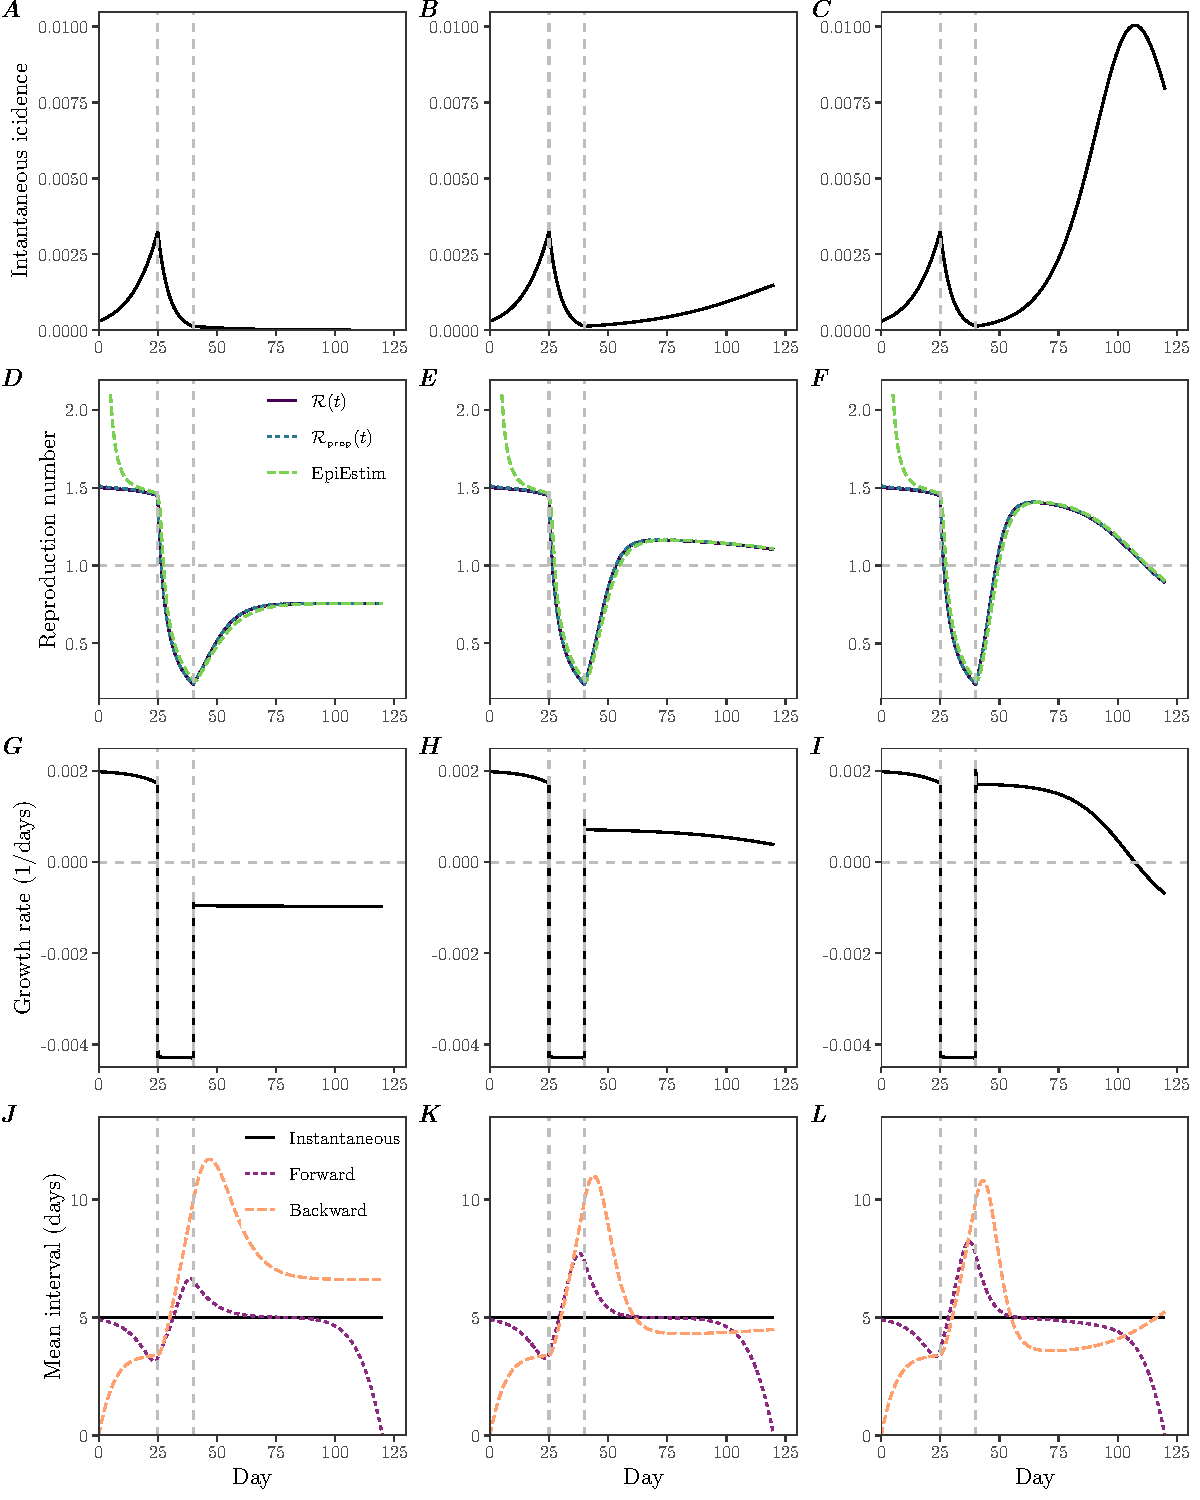
\includegraphics[width=\textwidth]{figure_sir_beta.pdf}
\caption{
\textbf{Epidemiological dynamics of a semi-mechanistic SIR model under equivalent constant-strength intervention.}
(A) Changes in true instantaneous reproduction number $\Ri(t)$, proportional reproduction number $\Rcori(t)$, estimated $\Ri(t)$ using EpiEstim (assuming a population of one million), and estimated $\tsub{\RR}{forward}(t)$ using the forward generation-interval distribution.
(B) Changes in true case reproduction number $\Rc(t)$, estimated $\Rc(t)$ using Wallinga-Teunis estimator with intrinsic generation-interval distribution, and estimated $\tsub{\RR}{forward}(t)$ using the forward generation-interval distribution.
(C) Changes in mean instantaneous, forward, and backward generation intervals.
}
\label{fig:sir_beta}
\end{figure}

Epidemiological dynamics under a constant-strength intervention are presented in \fref{sir_beta}.
In this case, the proportional reproduction number $\Rcori(t)$, which relies on the intrinsic generation-interval distribution, matches the instantaneous reproduction number $\Ri(t)$, which relies on the instantaneous generation-interval distribution (\fref{sir_beta}A).
Therefore, we are able to correctly estimate $\Ri(t)$ using \texttt{EpiEstim} (\fref{sir_beta}A).
The initial overestimation from \texttt{EpiEstim} is caused by the left censoring \citep{gostic2020practical}.
Minor differences between \texttt{EpiEstim} estimates and $\Rcori(t)$ are caused by discretization.

Likewise, we can accurately estimate the case reproduction number $\Rc(t)$ using the classic Wallinga-Teunis estimator (based on the intrinsic generation-interval distribution) (\fref{sir_beta}B).
This is because the instantaneous generation-interval distribution does not change over time under constant-strength interventions (\fref{sir_beta}C).
Using the forward generation-interval distribution, instead of the instantaneous generation-interval distribution, matches neither $\Ri(t)$ ($\tsub{\RR}{forward}(t)$ in \fref{sir_beta}A) nor $\Rc(t)$ in this case ($\tsub{\RR}{forward}(t)$ in \fref{sir_beta}B) because the forward distribution changes, even when the instantaneous distribution does not change (\fref{sir_beta}C).
As described earlier (\fref{indpop}A--C), introducing and lifting a constant-strength intervention cause the forward generation intervals become shorter and longer, respectively (\fref{sir_beta}C).
The backward distribution exaggerates these changes through the epidemic growth/decay effect---when an epidemic is growing (decaying), the mean backward intervals become shorter (longer).

\begin{figure}
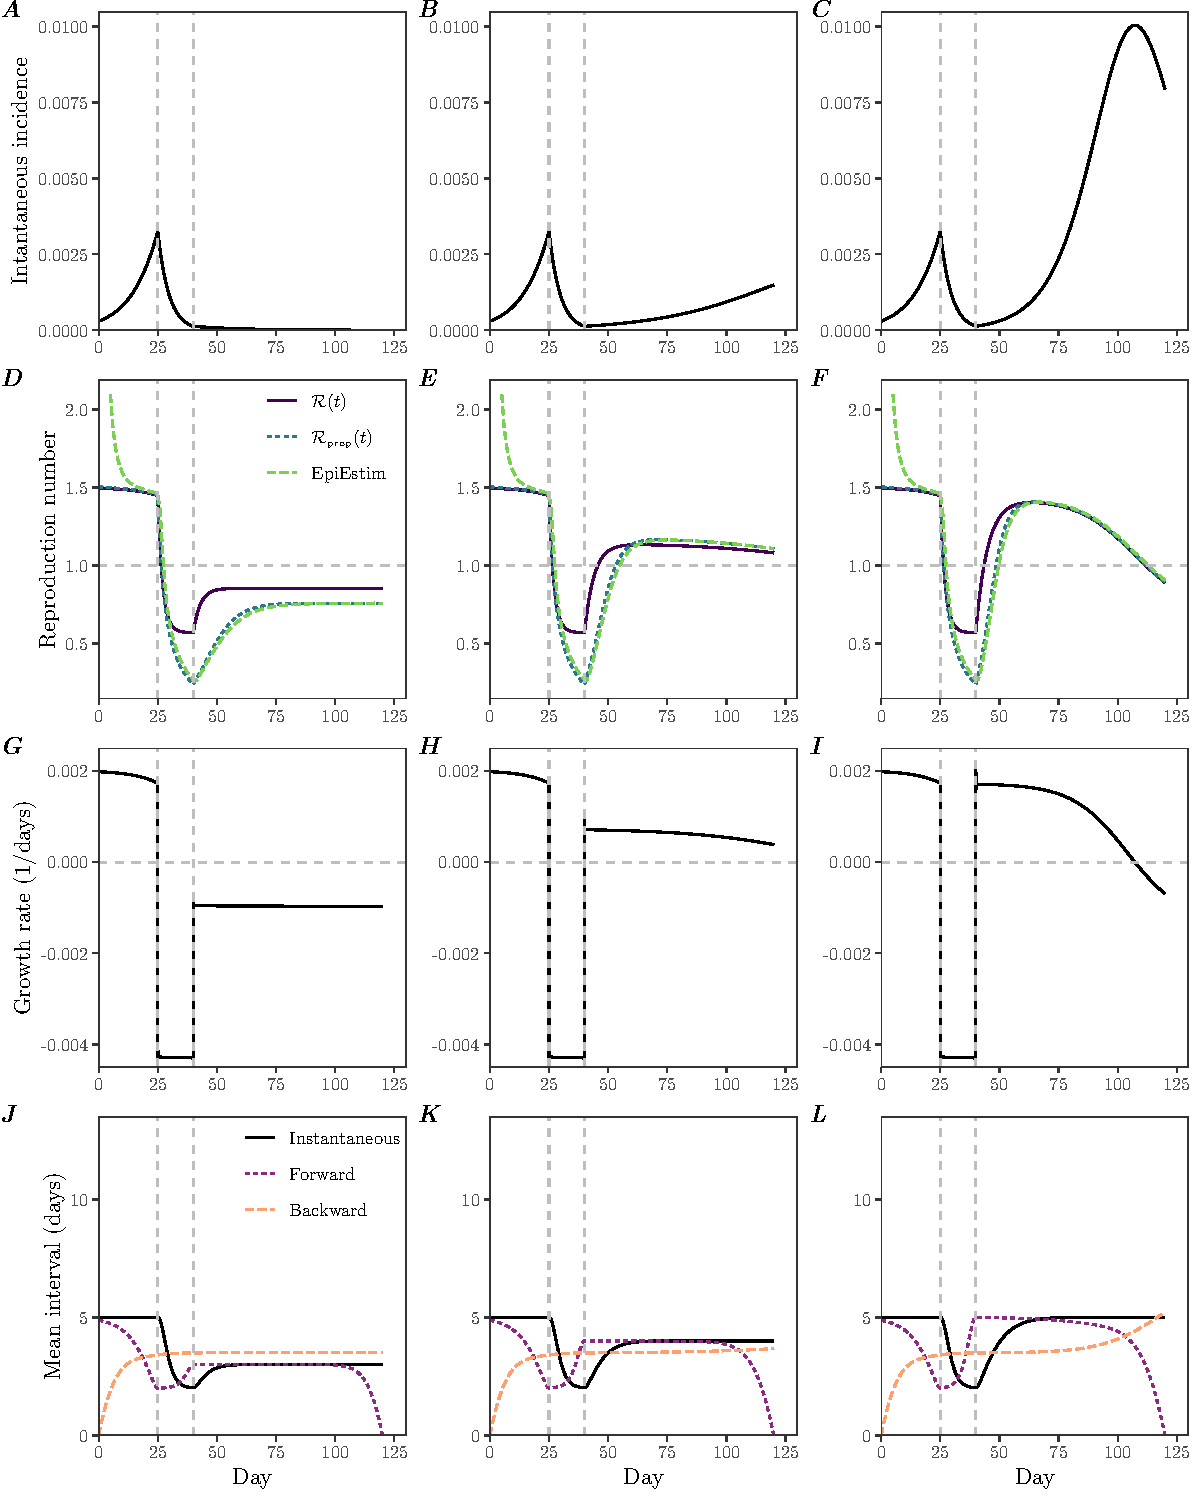
\includegraphics[width=\textwidth]{figure_sir_semi.pdf}
\caption{
\textbf{Epidemiological dynamics of a semi-mechanistic SIR model under equivalent constant-speed intervention.}
(A) Changes in true instantaneous reproduction number $\Ri(t)$, proportional reproduction number $\Rcori(t)$, estimated $\Ri(t)$ using EpiEstim (assuming a population of one million), and estimated $\tsub{\RR}{forward}(t)$ using the forward generation-interval distribution.
(B) Changes in true case reproduction number $\Rc(t)$, estimated $\Rc(t)$ using Wallinga-Teunis estimator with intrinsic generation-interval distribution, and estimated $\tsub{\RR}{forward}(t)$ using the forward generation-interval distribution.
(C) Changes in mean instantaneous, forward, and backward generation intervals.
}
\label{fig:sir_semi}
\end{figure}

Epidemiological dynamics under a constant-speed intervention are presented in \fref{sir_semi}.
In this case, the instantaneous generation-interval distribution changes through time.  
$\Rcori(t)$ differs from the true $\Ri(t)$ (\fref{sir_semi}A) because the constant-speed interventions lead to changes in the instantaneous generation-interval distribution (\fref{sir_semi}C).
Therefore, \texttt{EpiEstim} inaccurately estimates $\Ri(t)$ (\fref{sir_semi}A)---
in particular, \texttt{EpiEstim} estimates that $\Ri(t)$ crossed the threshold $\Ri(t)=1$ later (around $t=55$) than it actually did (around $t=45$).

Using the intrinsic distribution is also problematic for estimating the case reproduction number $\Rc(t)$ (\fref{sir_semi}B).
The true $\Rc(t)$ changes sharply, reflecting sharp changes in the removal rate $\gamma(t)$ (\fref{assumption}B), but using the intrinsic distribution gives smooth estimates of $\Rc(t)$.
In this case, $\tsub{\RR}{forward}(t)$ matches $\Ri(t)$ and $\Rc(t)$ better than their corresponding estimates using the intrinsic generation-interval distribution (EpiEstim and Wallinga-Teunis in \fref{sir_semi}, respectively) because the forward generation-interval distribution captures the effects of the constant-speed intervention (\fref{sir_semi}C).
Surprisingly, the backward generation-interval distribution stays nearly constant because the effect of decreasing incidence (which lengthens the backward generation intervals) cancels out with that of shorter realized generation intervals, caused by the constant-speed intervention (\fref{sir_semi}C).

Comparing simulations under equivalent constant-strength and constant-speed interventions allows us to better understand the differences between the $\Ri(t)$ and $r(t)$ in capturing current conditions at time $t$.
Under a constant-strength intervention, $\Ri(t) = \beta(t)/\gamma(0)$, and therfore $\Ri(t)$ crosses the threshold, $\Ri(t) = 1$, when $\beta(t)$ crosses the threshold, $\beta(t) = \gamma(0)$ (compare \fref{assumption}A with \fref{sir_beta}A).
Under a constant-speed intervention, however, sharp changes in $\gamma(t)$ translate to smooth changes in $\Ri(t)$, and therefore $\Ri(t)$ crosses the threshold, $\Ri(t) = 1$, later (compare \fref{assumption}B with \fref{sir_semi}A).
Instead, sharp changes in $\gamma(t)$ are captured by sharp changes in $r(t)$ (compare \fref{assumption}B with \fref{assumption}D)---this can readily seen by calculating $r(t)$ as the logarithmic derivative of the instantaneous incidence $i(t) = \beta(t) S I$.
\begin{equation}
r(t) =  \frac{1}{i(t)} \frac{\dd i(t)}{\dd t}\\
= \frac{1}{\beta(t)} \frac{\dd \beta(t)}{\dd t} - \beta(t) I + \beta(t) S - \gamma(t). \label{eq:explicitrt}
\end{equation}
\eref{explicitrt} also reinforces that the effect of changes in $\beta(t)$ on $r(t)$ are not straightforward, but are affected by per-capita changes in both $S$ and $I$.
Therefore, $\Ri(t)$ is a better measure for capturing current conditions at time $t$ under constant-strength interventions, whereas $r(t)$ is better for capturing current conditions at time $t$ under constant-speed interventions. 

\section{Discussion}

The impact of epidemic interventions are often characterized by changes in ``effective'' reproduction numbers, $\RR(t)$.
Many statistical softwares have been developed to accurately estimate $\RR(t)$, but the majority of existing frameworks neglect possibility that the underlying generation-interval distribution can change over time---an insight that goes back $>10$ years \citep{fraser2007estimating}.
Here, we distinguish two reproduction numbers---instantaneous reproduction number $\Ri(t)$ and case reproduction number $\Rc(t)$, which describe counterfactual and realized transmission processes, respectively---and show that both reproduction numbers can correctly describe the renewal process of infection when paired with correct generation-interval distributions.
In particular, a counterfactual distribution, which we call the instantaneous generation-interval distribution, is required to correctly estimate the instantaneous reproduction number. 
This distribution is affected by constant-speed, but not constant-strength, interventions.
Neglecting changes in this distribution gives biased estimates of $\Ri(t)$, including estimates of when $\Ri(t)$ crosses the threshold value of 1.
Instead, time-dependent growth rate $r(t)$ is a better measure for characterizing the impact of epidemic intervention under a constant-speed intervention.

In practice, estimating the instantaneous generation-interval distribution is expected to be difficult as it systematically differs from the realized generation intervals: even if we can observe all realized generation intervals throughout an epidemic, estimating the instantaneous distribution $g(t, \tau)$ is not trivial.
For example, even within a homogeneously mixing population, in which the disease is allowed to spread unchecked (and therefore $g(t, \tau) = g_0(\tau)$ for all $t$), aggregating all realized generation intervals underestimates the mean intrinsic generation interval due to susceptible depletion \citep{park2020inferring}.
Novel statistical methods are needed to accurately estimate the instantaneous distribution $g(t, \tau)$.

Most state-of-art statistical softwares for estimating reproduction numbers assume that the instantaneous generation-interval distribution does not change across time (e.g., \citep{10.12688/wellcomeopenres.16006.2,flaxman2020estimating,brauner2021inferring}).
We refer to these estimates as proportional reproduction numbers ($\Rcori$ above) as they capture proportional reduction in incidence, rather than transmission.
While this approach is parsimonious, practical and useful, it is important that researchers recognize the dependence on this assumption.
This reproduction number estimate can differ systematically from the true instantaneous reproduction number $\Ri$ under speed-like interventions such as contact tracing.
Emergence of variants with a different infectiousness profile (and therefore the intrinsic generation-interval distribution) can have similar effects.

In the context of the current SARS-CoV-2 pandemic, assuming a time-invariant generation-interval distribution was justifiable during the early period when most interventions were strength-like, including lockdowns, school closures, and travel bans \citep{flaxman2020estimating,li2021temporal,brauner2021inferring}.
Nonetheless, speed-like  interventions, including intense contact-tracing efforts \citep{park2020contact} and introduction of contact tracing apps \citep{wymant2021introduction}, had clear, non-negligible impact on the overall spread;
these interventions, including awareness-driven behavioral changes (which can cause symptomatic individuals to self-isolate faster), are likely to have shortened the instantaneous generation intervals by preventing transmission during later stages of infection.
Therefore, current estimates of $\Ri$ that rely on early estimates of the generation-interval distributions should be reassessed.
Future studies should also consider incorporating hazard-based changes for modeling speed-like interventions.

% \swp{return to this para}
% Our study highlights the value of growth rates $r(t)$ in characterizing epidemic spread \citep{abbott2020temporal,anderson2020reproduction}.
% The instantaneous reproduction number $\Ri(t)$ tell us whether the epidemic will continue to grow if conditions remain the same but does not tell us whether the epidemic is growing or not at a given moment.
% In contrast, $r(t)$ provides a robust measure of whether incidence is growing or decreasing at a given time under both strength- and speed-based interventions;
% but it does not provide information about future epidemic dynamics.
% \cite{parag2021epidemic} recently argued that $\RR(t)=1$ correspond to $r(t) = 0$ under correct assumptions about pathogen transmission and that $\RR(t)$ is theoretically more informative---however, we argue that this conclusion depends on their assumption to link $\RR(t)$ and $r(t)$ via the generation-interval distribution, an assumption that holds only when conditions remain constant.
% As we show here, this is not the case when conditions are changing---that is, the sign of $r(t)$ does not need to correspond to whether $\RR(t)$ is greater or less than 1.
% Time-varying reproduction number $\RR(t)$ and growth rate $r(t)$ encompass different information and should be used as complementary measures for describing epidemic dynamics \citep{dushoff2021speed}.

The renewal-equation framework based on the instantaneous form (\eref{renewal_instantaneous}) has been widely used in epidemic modeling due to its flexibility.
A few studies relied on the forward form (\eref{renewal_forward}), but they assumed a time-invariant generation-interval distribution \citep{nishiura2007time,alvarez2020variational,white2021statistical}.
As discussed above, the forward generation-interval distribution, which correctly links the case reproduction number with case counts, is expected to change over time.
To our knowledge, this is the first study to formally link the case reproduction number with the forward renewal equation and to demonstrate the equivalence between the forward and instantaneous renewal formulations.

This study highlights the complementary nature of time-varying reproduction number $\RR(t)$ and growth rate $r(t)$ as measures for describing epidemic dynamics \citep{dushoff2021speed}.
In particular, $r(t)$ can always be reliably estimated (given high-quality incidence data) but does not accurately reflect changes in current conditions, except when changes are predominantly speed-like.
Conversely, $\RR(t)$ -- and particularly the instantaneous reproductive number $\Ri(t)$ -- provides an accurate reflection of current conditions in \emph{theory}, but can only be reliably estimated from incidence data alone when changes are primarily strength-like.
Methods that use real-time information about \emph{changes} in disease-transmission intervals have the potential to unify these frameworks, but will often be limited by the difficulty of collecting sufficient high-quality data.

\section{Methods}

\subsection{Equivalent constnat-strength and constant-speed interventions}

We model a simple scenario in which a flu-like pathogen with $\Ro = 1.5$ invades an immunologically naive population using the semi-mechanistic SIR model (\eref{dSdt}--\eref{dRdt}).
We begin by modeling constant-speed intervention and find the equivalent constant-strength intervention.  
In particular, we assume that the disease spreads without any intervention in the beginning;
on day 25, an intense case isolation measure is implemented; and
on day 40, the intervention is partially lifted.
This is modeled as follows:
\begin{equation}
\beta(t) = 0.3\,\,\textrm{days}^{-1}, \gamma(t) = \begin{cases}
0.2\,\, \textrm{days}^{-1} & t < 25\\
0.5\,\, \textrm{days}^{-1} & 25 \leq t < 40 \\
0.25\,\, \textrm{days}^{-1} & 40 \leq t
\end{cases}.
\end{equation}
Simulations are run for 100 days based on the following initial conditions: $S(0) = 1 - 10^{-3}$, $I(0) = 10^{-3}$, and $R(0) = 0$.

Since we assume that incidence is known exactly until time $t^\ast$ we can estimate the transmission rate $\beta^\ast(t)$ (with fixed $\gamma(t)=\gamma(0)$) that gives an identical incidence trajectory until time $t < t^\ast$.
This transmission rate is given by:
\begin{equation}
\beta^\ast(t) = \frac{\Rcori(t)\gamma(0)}{S(t)},
\end{equation}
where the proportional reproduction number $\Rcori$ is calculated from the incidence curve $i(t)$ for time $t < t^\ast$.
More generally, given true incidence $i(t)$ until time $t^\ast$, modulated by any interventions, we can find equivalent constant-strength intervention $\PP^\ast(t)$ until time $t^\ast$:
\begin{equation}
\PP^\ast(t) = \frac{\Rcori(t)}{\Ro S(t)},
\end{equation}
which generates an identical incidence curve when the initial conditions are identical.

\pagebreak

\section*{Supplementary Materials}
\setcounter{figure}{0}
\renewcommand{\thefigure}{S\arabic{figure}}


\begin{figure}[!th]
\includegraphics[width=1\textwidth]{pop_ind_compare_inst.pdf}
\caption{
\textbf{The impact of constant-strength and constant-speed interventions on instantaneous kernels.}
The impact of constant-strength (A--C) and constant-speed (D--F) intervention on instantaneous kernels at different time:
5 days before intervention onset (A, D), during intervention (B, E), and 5 days before intervention offset (C, F).
Gray shaded curves represent the (fixed) intrinsic kernel $K_0(\tau)$, which is modeled using a gamma distribution with $\Ro$ of 2, a mean of 5 days and a squared coefficient of variation of 0.2.
Colored curves represent the instantaneous kernel $K(t, \tau)$ under constant-strength (A--C) and constant-speed (D--F) interventions.
The constant-strength intervention is assumed to reduce kernel by a factor of 2.
The constant-speed intervention is assumed to have a constant hazard of $1/5/\textrm{days}$ during the intervention period.
Susceptible depletion is assumed to be negligible.
Solid black lines represent relative changes in the kernel: $K(t, \tau)/K_0(\tau)$.
Solid vertical lines show the (fixed) mean intrinsic generation interval and dashed vertical lines the mean instantaneous generation interval.
}
\end{figure}

\pagebreak

\bibliography{individual_intervention}



\end{document}
